% !TeX root = ../../main.tex
% ------------------------------------------------------------------
%  Arquitectura de despliegue
%  Fragmento del Subdocumento 4.2, traido desde contenido.tex con
%  \parte{partes/11_j_despliegue}. Las rutas son relativas a la carpeta del
%  subdocumento, nunca a la de main.tex.
%
%  Complementa la sección de conexiones y puntos de falla.
% ------------------------------------------------------------------

% Mini título de cada ambiente: sin número, no entra al índice.
\providecommand{\minititulo}[1]{\par\addvspace{8pt}\noindent{\intersemibold\color{lafroxTinta}#1}\par\nopagebreak\addvspace{2pt}}

\section{Arquitectura de despliegue}
\label{sec:despliegue}

La arquitectura física describe qué componentes existen, dónde viven y cómo se conectan. Esta sección describe cómo esa solución se pone en marcha y se mantiene en operación durante los 56 meses del contrato: por qué ambientes pasa un cambio antes de llegar a las bodegas y a la calle, sobre qué red se despliega, cómo sigue operando cuando algo falla y cómo se recupera cuando se pierde un sitio completo o se daña un dato. Los puntos de falla de cada conexión y de cada equipo, con su resolución inmediata, se declaran en la sección de conexiones y contingencia (Tablas~\ref{tab:fallas-sitios} y~\ref{tab:fallas-nube}). Aquí se describen los mecanismos que sostienen esa continuidad y cómo se verifican.

Esos mecanismos son tres y no se sustituyen entre sí. La alta disponibilidad responde a la falla de un componente sin que la operación lo note. La recuperación ante desastres responde a la pérdida de un sitio o de una región completa. El respaldo responde al daño del dato, sea un borrado accidental, una corrupción o un cifrado malicioso, frente a los cuales las réplicas no protegen, porque replican el daño con la misma fidelidad que una escritura legítima.

\subsection{Ambientes y ciclo de entrega}
\label{sub:1-ambientes-de-despliegue-rt-04-01}

Un cambio recorre tres ambientes antes de llegar a Producción: Desarrollo, QA y Preproducción. Se construye y se prueba de forma unitaria en Desarrollo, se valida en QA con pruebas funcionales, de integración y de regresión automatizadas, y se ensaya en Preproducción, donde ocurren las pruebas de aceptación, de carga y de resiliencia y el ensayo del paso a producción. Solo entonces se promueve a Producción, sin recompilar, de modo que el artefacto que llega a producción es el mismo que se probó. La marcha blanca de cada etapa ocurre ya en Producción, porque es operación supervisada con datos y usuarios reales en paralelo con la operación vigente. Un quinto ambiente, de Recuperación ante Desastres, sostiene la continuidad: reside en la región us-east-1 para el dominio de nube, mientras que el WMS de Talca se recupera en la plataforma de nube, como se describe en la recuperación ante desastres de esta sección. La Tabla~\ref{tab:t62} muestra cada ambiente con su bloque de direccionamiento, su región y su función.

\begin{tablalafrox}{Ambientes de despliegue}{tab:t62}%
  {F{0.28} F{0.20} F{0.15} Y}%
  {\cab{Ambiente} & \cab{VPC} & \cab{Región} & \cab{Función}}
  Desarrollo & 10.104.0.0/16 & sa-east-1 & Construcción y pruebas unitarias \\
  QA & 10.103.0.0/16 & sa-east-1 & Pruebas funcionales, de integración y de regresión, y análisis dinámico \\
  Preproducción & 10.102.0.0/16 & sa-east-1 & Aceptación, carga, resiliencia y ensayo del paso a producción \\
  Producción & 10.101.0.0/16 & sa-east-1 & Operación en varias zonas, con los sitios on-premise, y marcha blanca \\
  Recuperación ante Desastres & 10.201.0.0/16 & us-east-1 & Réplica en caliente del dominio de nube y recuperación del WMS de Talca en la nube \\
\end{tablalafrox}

{\footnotesize Fuente: elaboración propia.\par}

Cada ambiente reside en una cuenta AWS propia, bajo una organización de AWS Control Tower cuyas políticas de control de servicio impiden que un error o un acceso indebido en un ambiente alcance a otro. La organización incorpora además sus cuentas de gestión, de archivo de registros y de auditoría. Los bloques de direccionamiento no se solapan entre sí ni con los de los sitios on-premise, y solo el ambiente de recuperación reside fuera de la región primaria. Los cinco ambientes quedan habilitados y operativos en el hito H3 del Formulario E-25, en el mes 6 del contrato, antes de la primera marcha blanca (RT-04.01; Bases Técnicas Transversales, cap. 4, p. 10).

En la nube, en los cinco ambientes, la imagen de la aplicación corre en ECS Fargate, que es el cómputo de la plataforma de aplicación N-04 (Tabla~\ref{tab:servicios-nube}). Cada ambiente despliega la imagen en su propia cuenta, desde el mismo Elastic Container Registry de sa-east-1, que replica cada imagen en us-east-1 para que la región de recuperación no dependa de la primaria. Los ambientes se diferencian en su escala y en su conectividad, no en el servicio donde corre el código:

\begin{itemize}
  \item Producción opera en dos zonas.
  \item Preproducción replica esa topología.
  \item Desarrollo, QA y Preproducción se reducen o apagan fuera del horario de uso.
  \item Recuperación ante Desastres mantiene la réplica reducida de us-east-1.
\end{itemize}

Desarrollo y QA son aislados y se reconstruyen desde código. Desarrollo trabaja con datos sintéticos o anonimizados, y QA con un juego de datos de prueba controlado y versionado que se restituye a un estado conocido antes de cada ciclo de pruebas. Ningún ambiente no productivo recibe datos productivos sin anonimización o seudonimización verificable. Desarrollo, QA y Preproducción se reducen o apagan fuera del horario de uso, con el ahorro reflejado en la estructura de costos (RT-04.13; Bases Técnicas Transversales, cap. 4, p. 11).

Las bodegas no tienen ambientes propios de prueba, y no los necesitan. El on-premise es producción: la imagen wms\_only que corre en los centros de distribución y en los cross-docking es la misma que recorrió Desarrollo, QA y Preproducción en la nube, y la infraestructura de cada sitio se declara como código versionado. Lo que se ensayó en la nube es, por lo tanto, lo que se instala en Talca, en Concepción y en cada cross-docking, sitio por sitio. QA y Preproducción ensayan esa imagen con el verificador local de identidad y la puerta de API local del WMS, con adaptadores simulados del ERP, y reproducen el corte de enlace y el relevo de turno antes de cada paso a producción.

Preproducción es equivalente a Producción en versiones, configuración, dimensionamiento y topología de nube (RT-04.02; Bases Técnicas Transversales, cap. 4, p. 10). Subsisten tres diferencias justificadas:

\begin{enumerate}
  \item Preproducción se reduce o apaga fuera del horario de uso, por costo.
  \item Preproducción trabaja con datos sintéticos generados desde la volumetría del caso, cuya anonimización se verifica con Amazon Macie, porque no se admiten datos productivos reales fuera de Producción sin anonimización verificable.
  \item Preproducción emula el sitio on-premise dentro de su propia VPC, con la misma imagen wms\_only, el mismo broker y el mismo verificador local, pero sin túnel hacia las bodegas, para que un ensayo no pueda alcanzar la operación real.
\end{enumerate}

La emulación reproduce la topología del sitio y no su hardware. Por eso, la primera instalación de cada entrega en los centros de distribución y los cross-docking avanza sitio por sitio, como se describe en la liberación. Durante las pruebas de carga y estrés de la Tabla~\ref{tab:t86} opera con el dimensionamiento completo de Producción.

Las figuras siguientes muestran cada uno de los cinco ambientes. Desarrollo, QA y Preproducción residen solo en la nube. Producción abarca la nube y los sitios on-premise. Recuperación ante Desastres cubre la pérdida de la región primaria mediante us-east-1 y la pérdida de la sala de Talca mediante el WMS levantado en la plataforma de nube (numeral 4.1 de las Bases Técnicas Transversales; Bases Técnicas Transversales, cap. 4, p. 10). Concepción opera su propia bodega en Producción.

\minititulo{Desarrollo}

La Figura~\ref{fig:amb-desarrollo} muestra cómo llega una entrega a Desarrollo. Sus pasos numerados se leen de izquierda a derecha.

\begin{figure}[htbp]\centering
  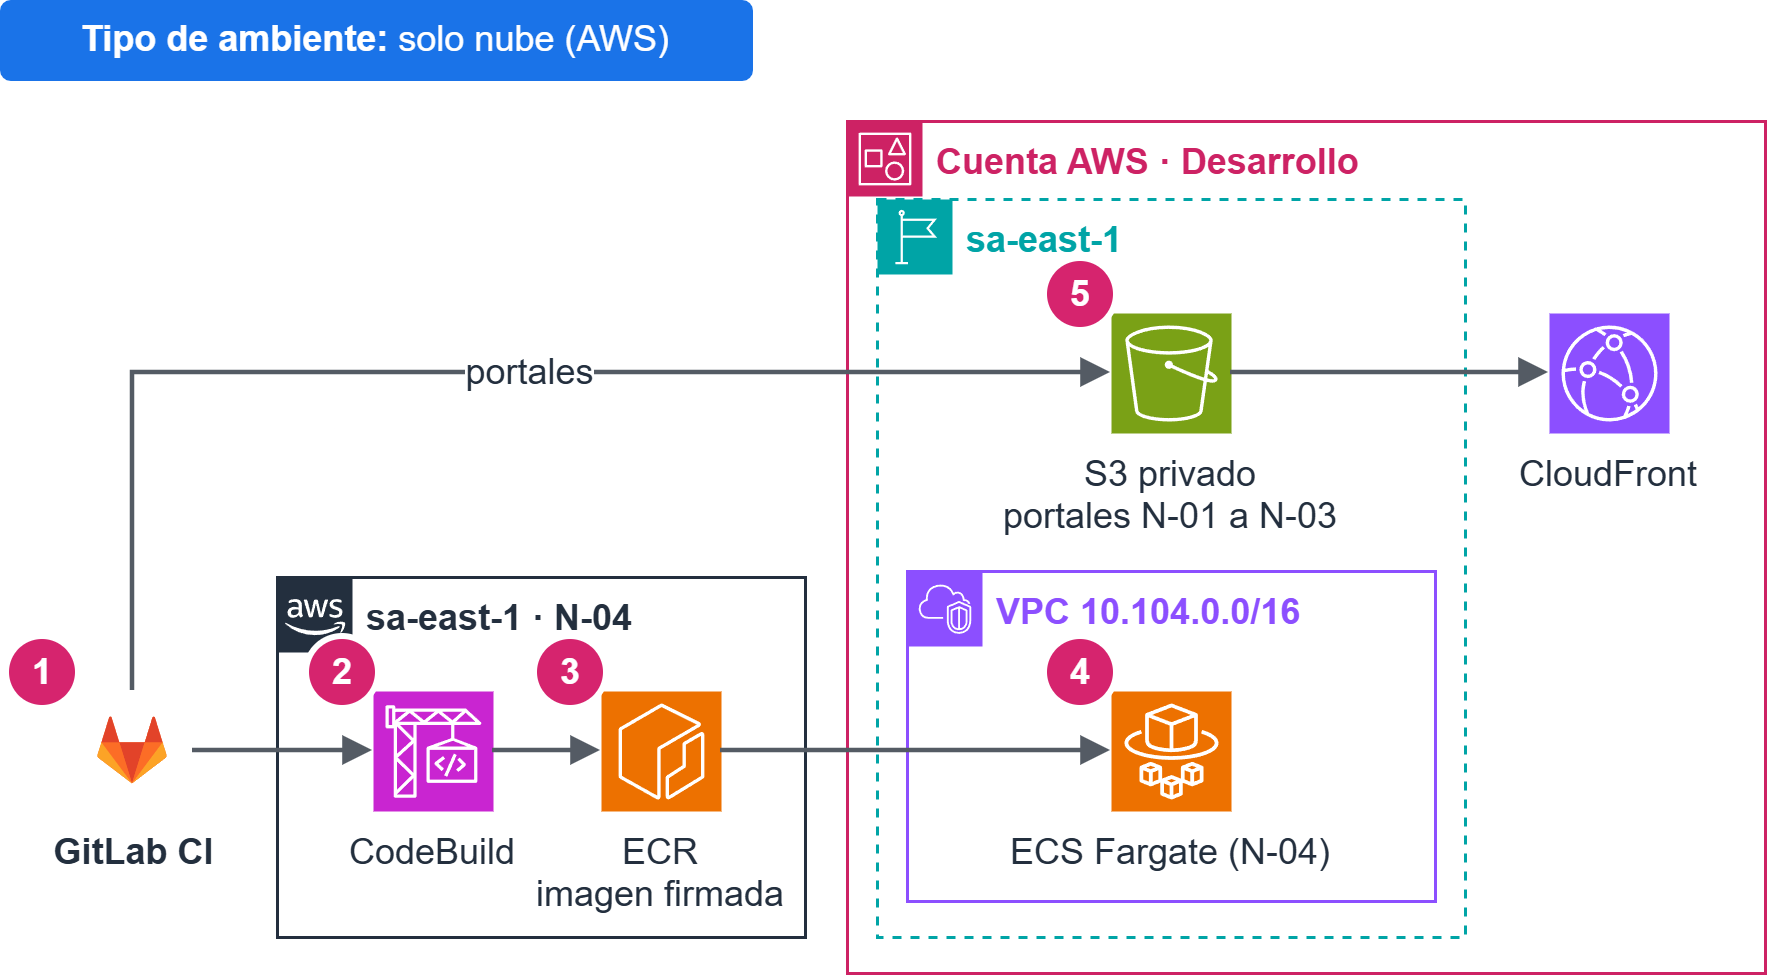
\includegraphics[width=\textwidth]{figuras/fisica/ambientes/amb_desarrollo.png}
  \caption{Ambiente de Desarrollo}\label{fig:amb-desarrollo}
  \fuentefigura
\end{figure}
\FloatBarrier

Los pasos de la figura son los siguientes:

\begin{enumerate}
  \item GitLab CI toma el cambio aprobado en la rama protegida y ejecuta los controles del pipeline, que se detallan más adelante en esta sección.
  \item AWS CodeBuild construye la imagen de la aplicación una sola vez, de forma hermética y con procedencia SLSA nivel 3.
  \item Elastic Container Registry (ECR) guarda la imagen firmada. Desde aquí se promueve por su digest a los demás ambientes, sin recompilar.
  \item ECS Fargate despliega la imagen en la VPC 10.104.0.0/16 de la cuenta de Desarrollo, con la configuración de SSM Parameter Store y los secretos de AWS Secrets Manager propios del ambiente.
  \item El pipeline publica los portales Angular de clientes, transportistas y proveedores (N-01 a N-03) en un bucket S3 privado, que CloudFront sirve.
\end{enumerate}

Desarrollo no tiene enlace con los sitios.

\minititulo{QA}

QA repite la secuencia de Desarrollo en su propia cuenta y su propia VPC (Figura~\ref{fig:amb-qa}). No construye una imagen nueva: usa la misma que recorrió Desarrollo, de modo que una falla detectada aquí corresponde al artefacto y no a una recompilación.

\begin{figure}[htbp]\centering
  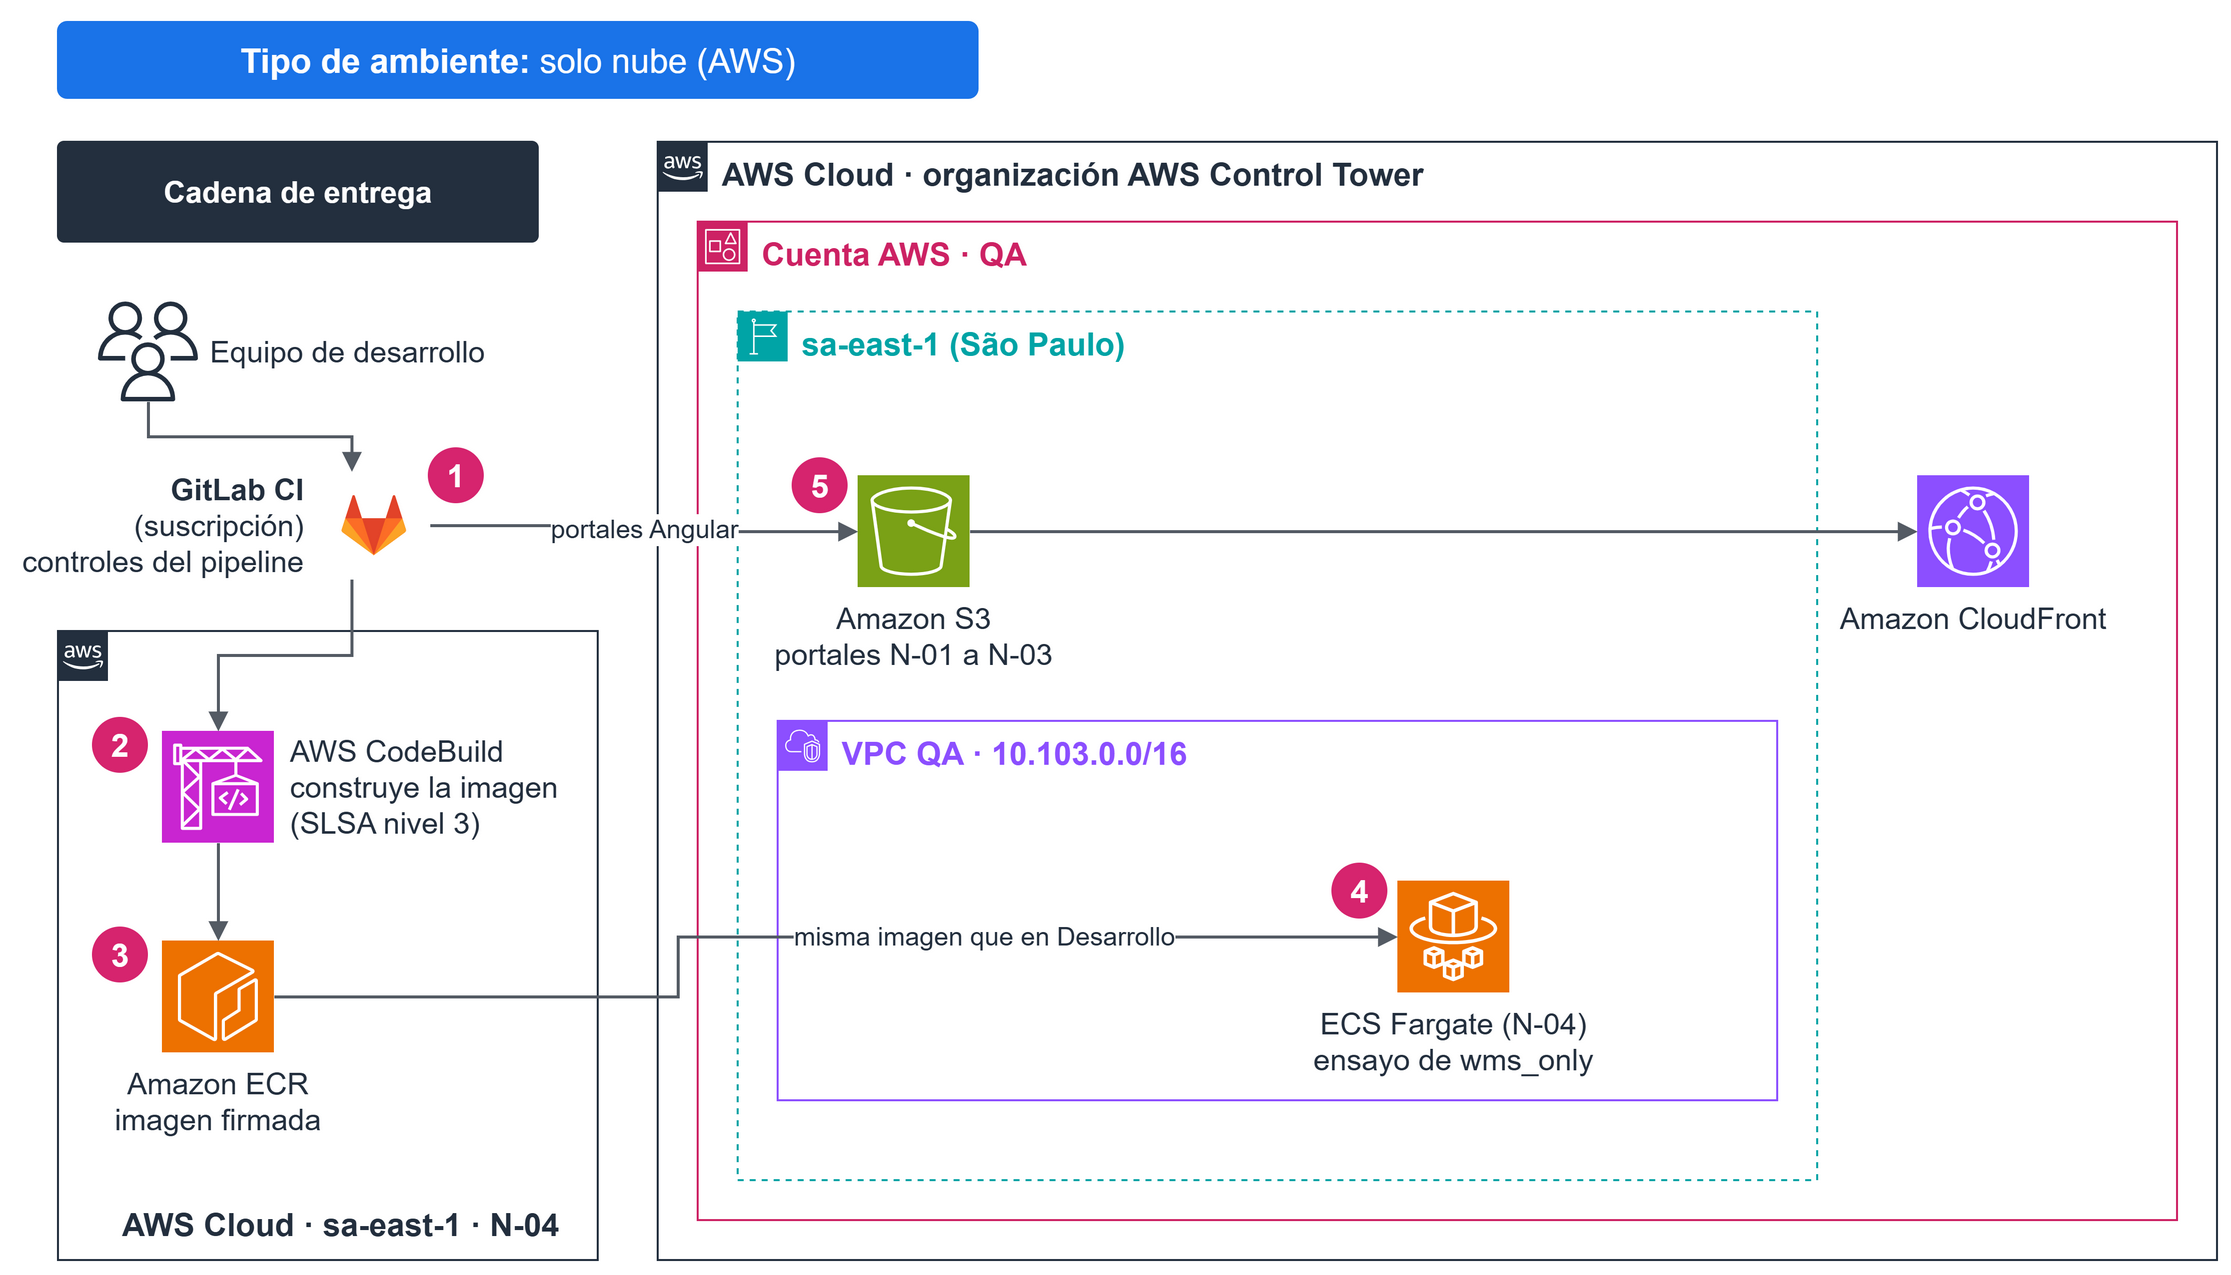
\includegraphics[width=\textwidth]{figuras/fisica/ambientes/amb_qa.png}
  \caption{Ambiente de QA}\label{fig:amb-qa}
  \fuentefigura
\end{figure}
\FloatBarrier

Los pasos de la figura son los siguientes:

\begin{enumerate}
  \item GitLab CI promueve a QA la entrega que superó Desarrollo.
  \item CodeBuild no vuelve a construir: la imagen es la que construyó para Desarrollo.
  \item ECR entrega esa imagen firmada, identificada por su digest.
  \item ECS Fargate la despliega en la VPC 10.103.0.0/16 de la cuenta de QA, donde corren las pruebas funcionales, de integración y de regresión.
  \item Los portales se publican en el bucket S3 privado de QA, que CloudFront sirve.
\end{enumerate}

\minititulo{Preproducción}

En Preproducción la secuencia se ensaya sobre la topología de Producción y sobre un sitio on-premise emulado (Figura~\ref{fig:amb-preproduccion}). Aquí se demuestran las migraciones y el despliegue azul-verde con canario antes de cada paso a producción (RT-04.07; Bases Técnicas Transversales, cap. 4, p. 11).

\begin{figure}[htbp]\centering
  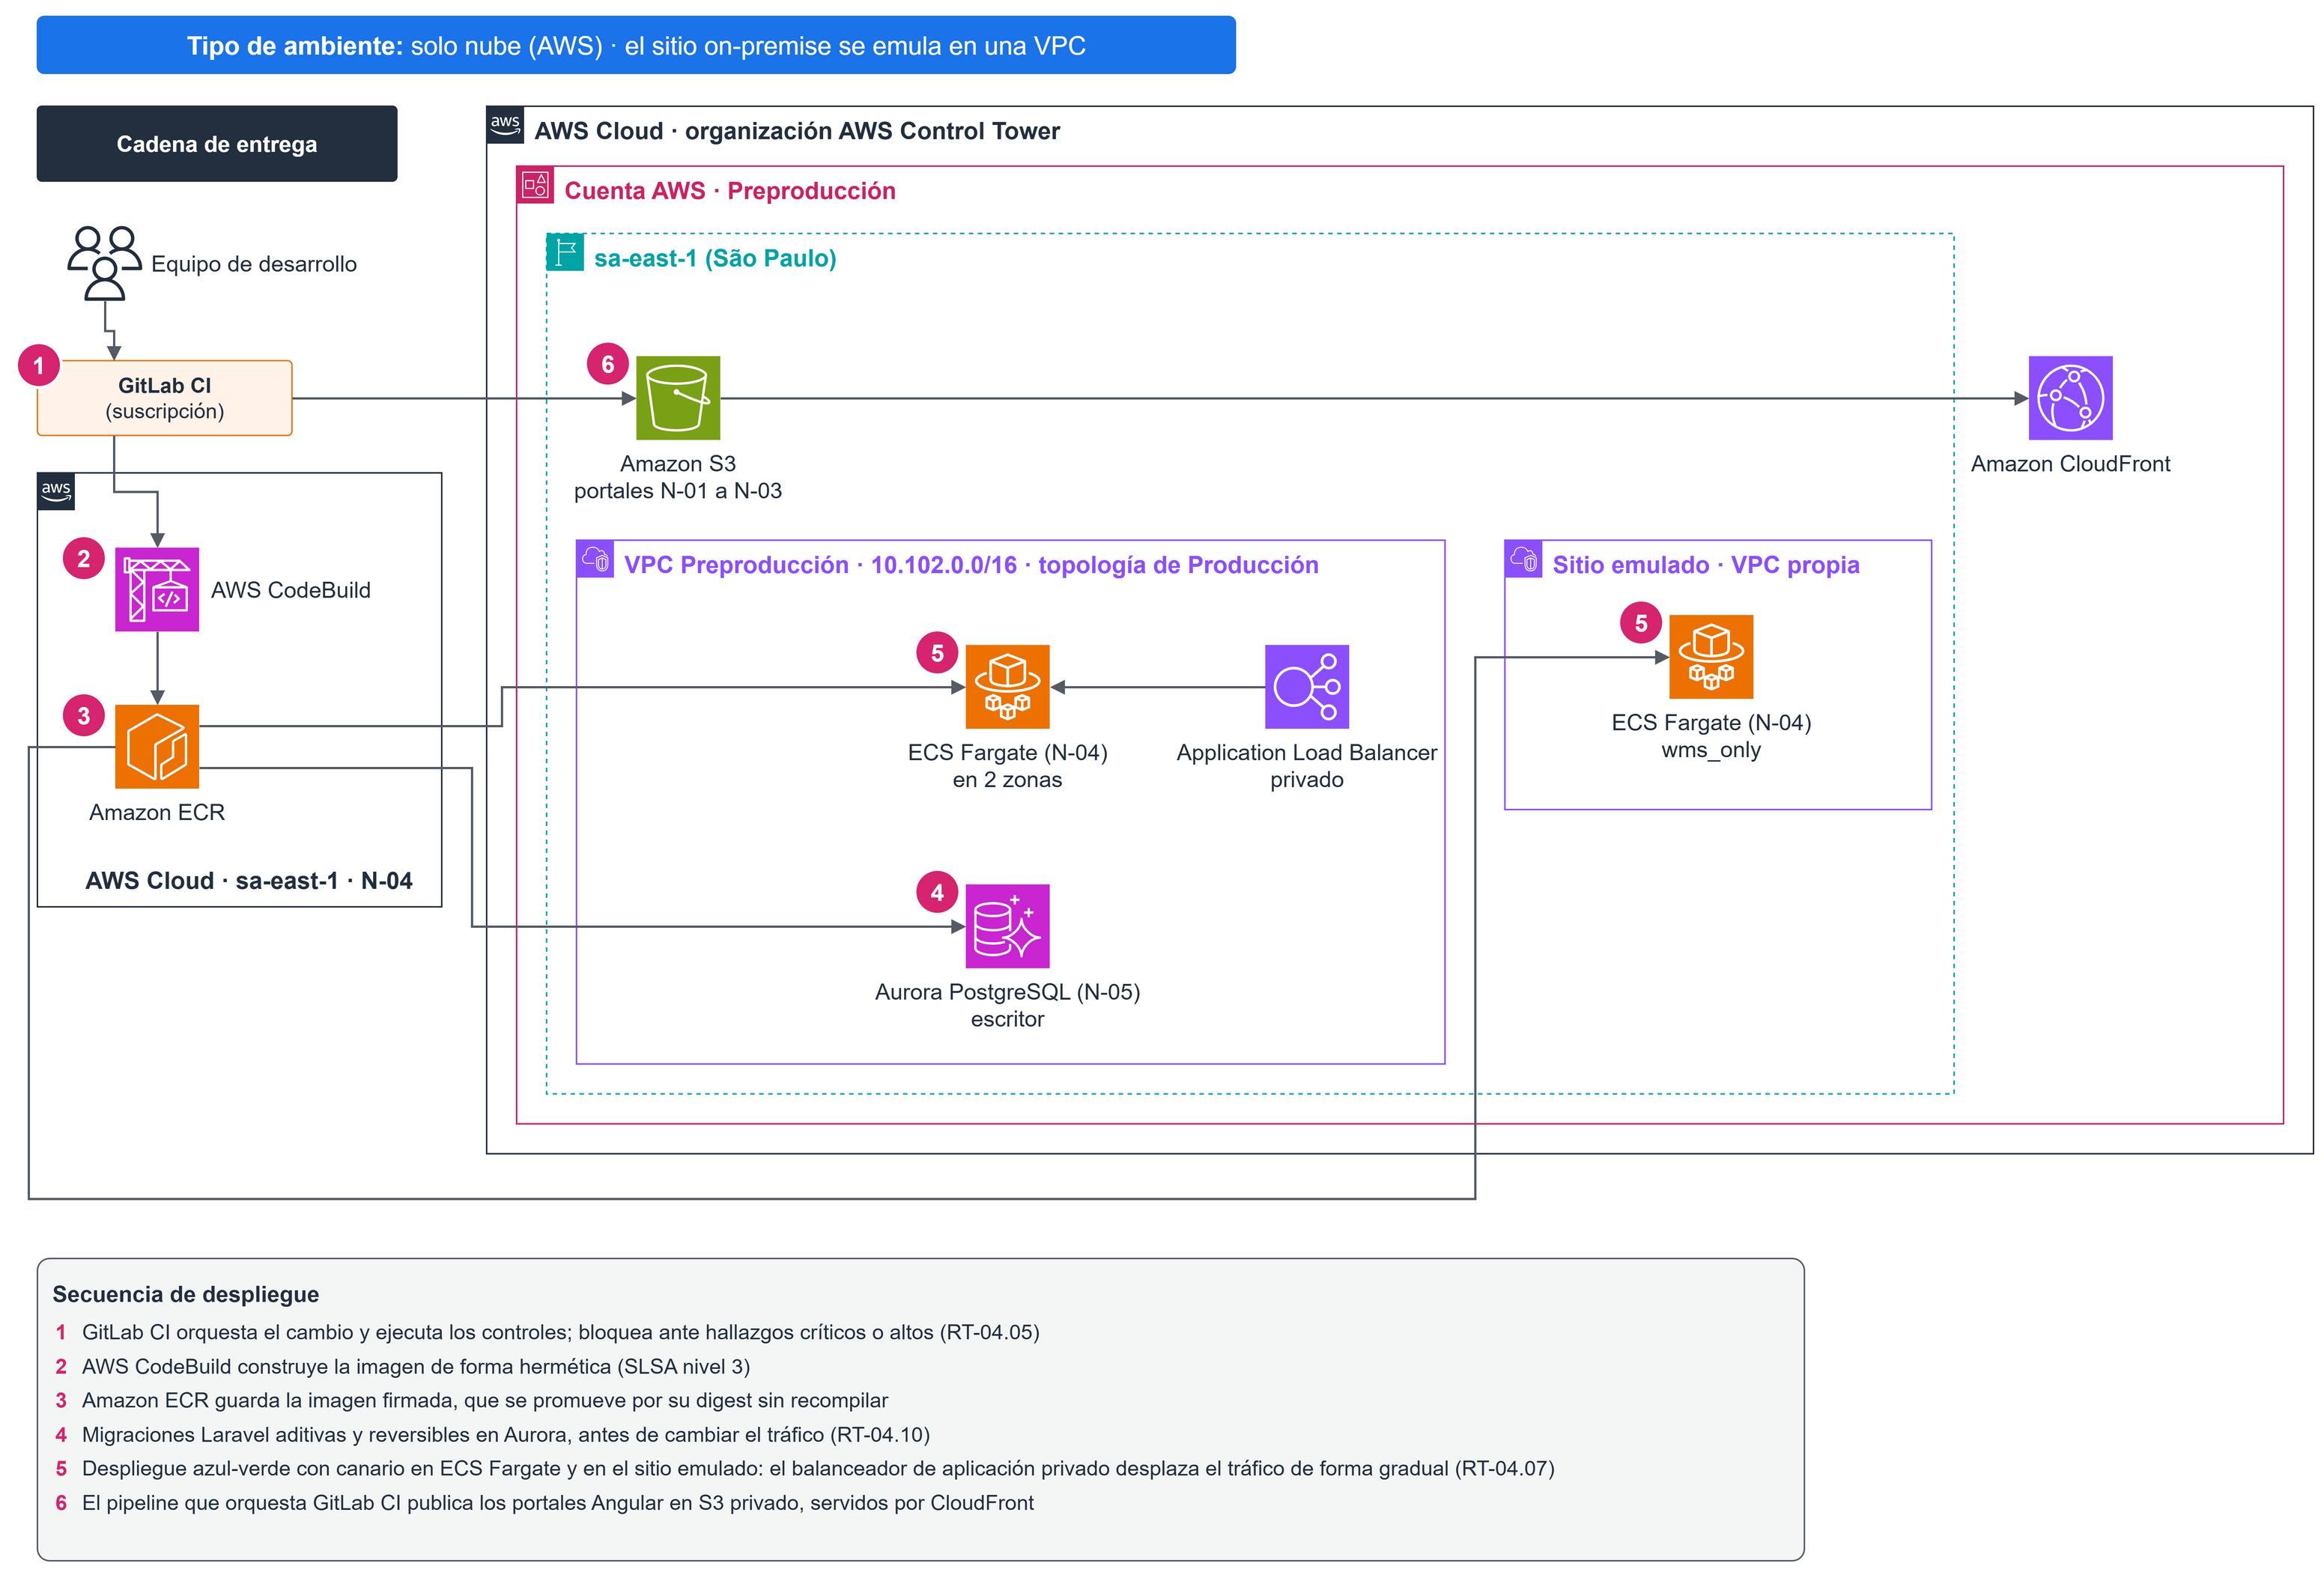
\includegraphics[width=\textwidth]{figuras/fisica/ambientes/amb_preproduccion.png}
  \caption{Ambiente de Preproducción}\label{fig:amb-preproduccion}
  \fuentefigura
\end{figure}
\FloatBarrier

Los pasos de la figura son los siguientes:

\begin{enumerate}
  \item GitLab CI promueve a Preproducción la entrega que superó QA.
  \item CodeBuild no vuelve a construir: la imagen es la misma de Desarrollo y QA.
  \item ECR entrega la imagen firmada por su digest.
  \item Las migraciones aditivas se aplican sobre el escritor de Aurora PostgreSQL (N-05), como un paso único antes de cambiar el tráfico.
  \item La entrega nueva se despliega al mismo tiempo en dos lugares, por lo que la figura asigna el número 5 a ambos:
  \begin{itemize}
    \item En la VPC 10.102.0.0/16 se ensaya el despliegue azul-verde con canario. La entrega vigente («azul») sigue atendiendo mientras ECS Fargate levanta la nueva («verde») a su lado. El balanceador privado, en dos zonas, le pasa primero a la nueva una parte pequeña del tráfico, llamada canario, y la aumenta por etapas mientras no aparezcan errores. Si aparecen, el tráfico vuelve completo a la entrega vigente.
    \item En la VPC del sitio emulado, su base local recibe las mismas migraciones aditivas y la imagen \texttt{wms\_only} recibe la misma entrega mientras el sitio está desconectado. Al reconectarlo, se comprueba que la reconciliación acepta los sobres que dejó la entrega previa.
  \end{itemize}
  \item Los portales se publican en el bucket S3 privado de Preproducción, que CloudFront sirve.
\end{enumerate}

La VPC del sitio emulado no tiene túnel hacia las bodegas, de modo que ningún ensayo alcanza la operación real.

\minititulo{Producción}

En Producción la secuencia se ejecuta de forma automática y llega además a los sitios on-premise (Figura~\ref{fig:amb-produccion}).

\begin{figure}[!htbp]\centering
  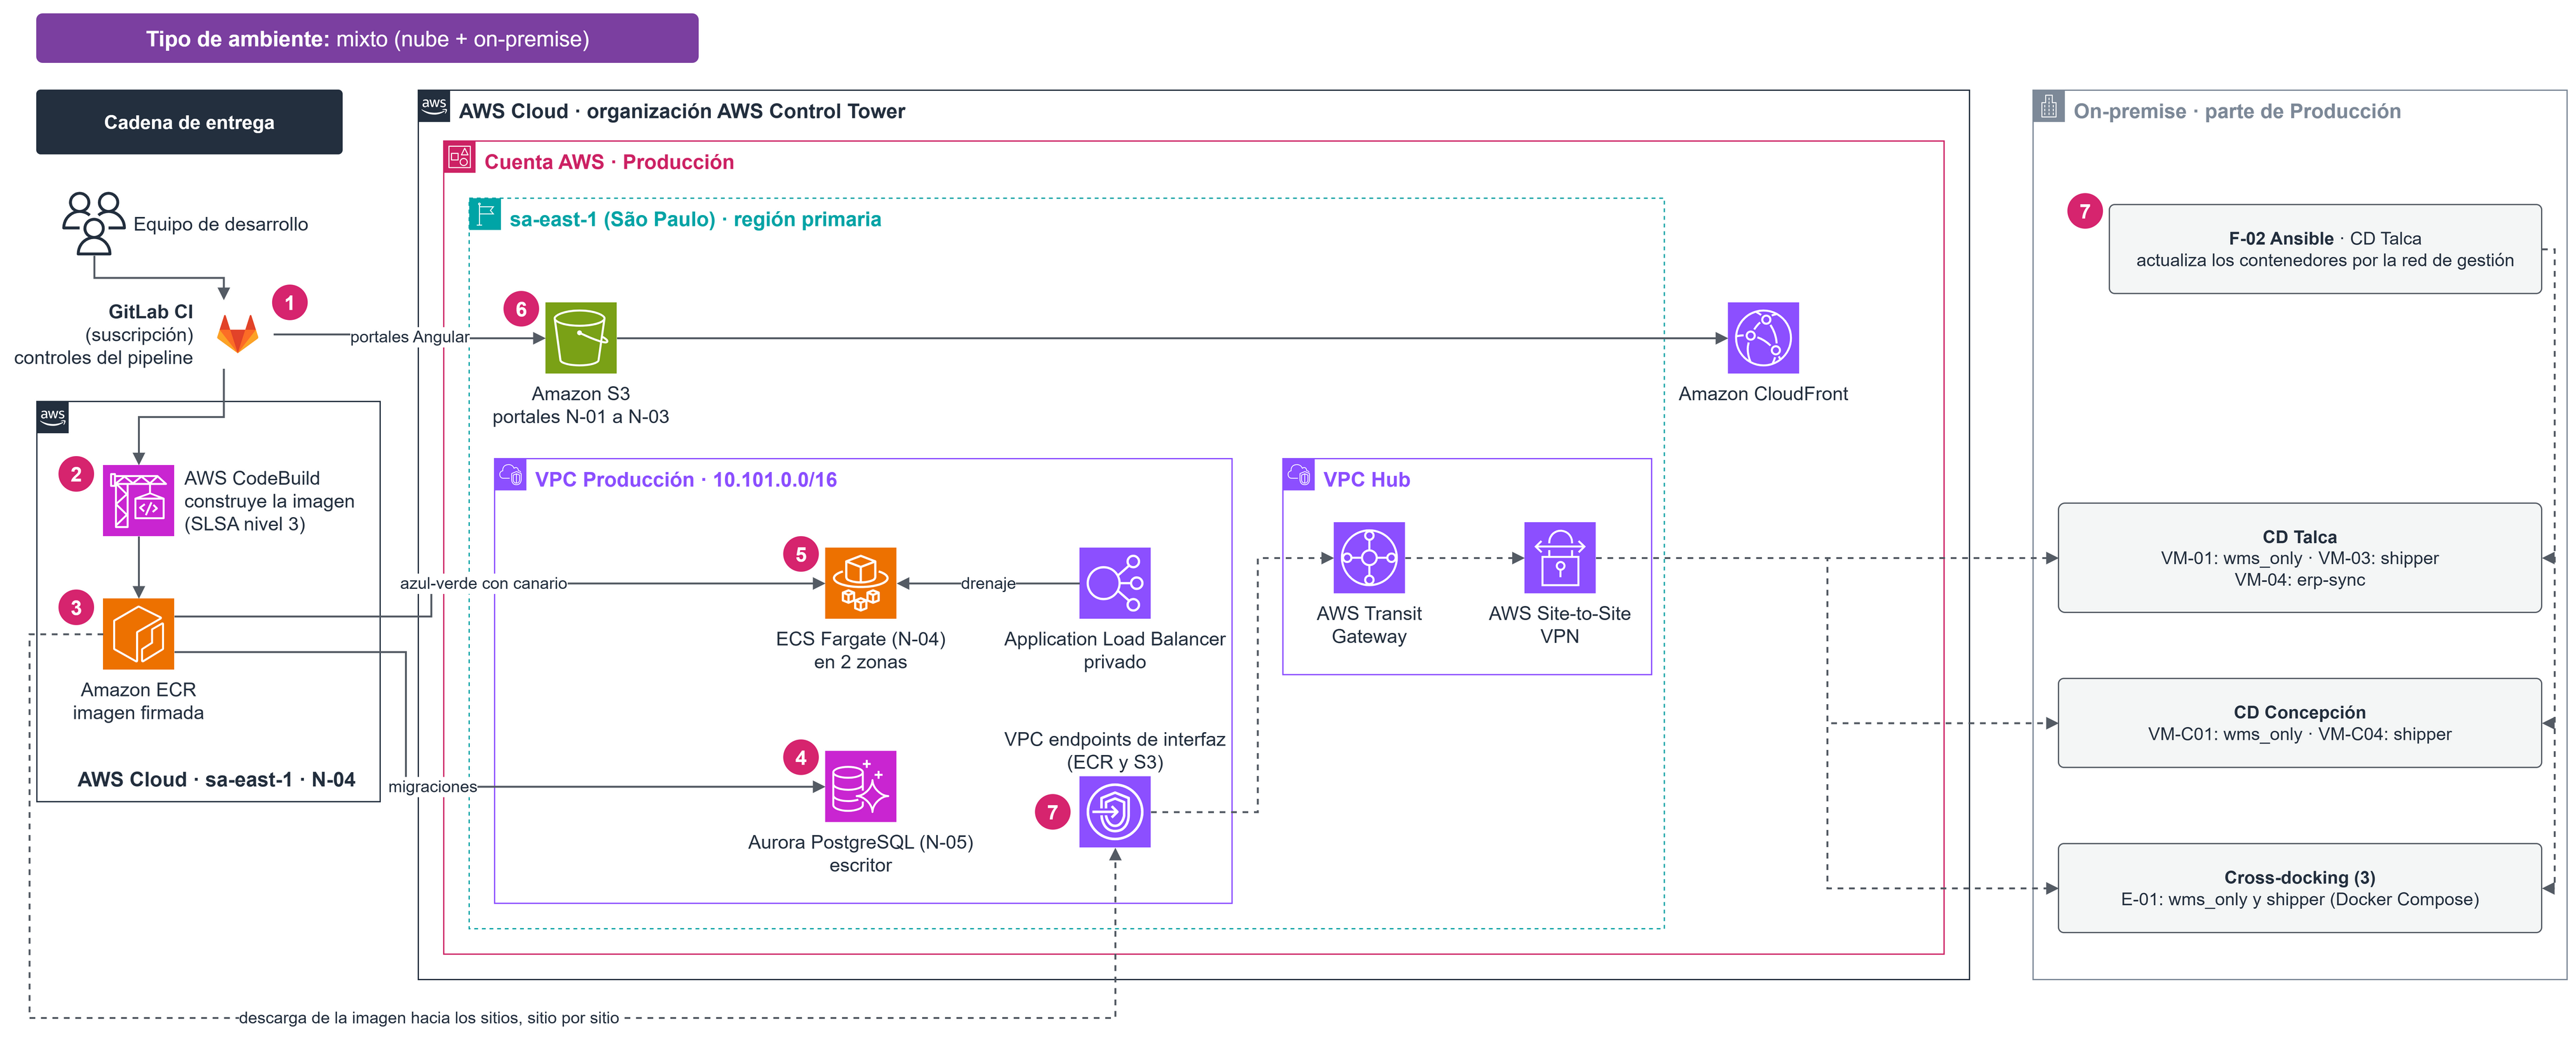
\includegraphics[width=\textwidth]{figuras/fisica/ambientes/amb_produccion.png}
  \caption{Ambiente de Producción}\label{fig:amb-produccion}
  \fuentefigura
\end{figure}

\FloatBarrier

Los pasos de la figura son los siguientes:

\begin{enumerate}
  \item GitLab CI inicia el paso a producción cuando la entrega superó los controles del pipeline y el ensayo en Preproducción, dentro de las ventanas de la Tabla~\ref{tab:jd02}.
  \item CodeBuild no vuelve a construir: la imagen es la misma que se ensayó.
  \item ECR entrega la imagen firmada por su digest.
  \item Las migraciones aditivas se aplican sobre el escritor de Aurora PostgreSQL (N-05).
  \item ECS Fargate aplica en la VPC 10.101.0.0/16, en dos zonas, el mismo despliegue azul-verde con canario que se ensayó en Preproducción: la entrega nueva recibe el tráfico por etapas y, si falla, el tráfico vuelve a la vigente.
  \item Los portales se publican en el bucket S3 privado de Producción, que CloudFront sirve.
  \item La entrega llega a los sitios mediante dos acciones que ocurren juntas, por lo que la figura asigna el número 7 a ambas:
  \begin{itemize}
    \item Los sitios descargan la misma imagen desde ECR por la VPN, la VPC Hub y los endpoints de interfaz de la VPC de Producción, en conexiones salientes y sin pasar por Internet.
    \item Ansible (F-02), desde CD Talca, aplica sitio por sitio las migraciones aditivas a la base PostgreSQL activa: VM-02, VM-C02 y la del E-01 activo. En Concepción y los cross-docking, la réplica sincrónica las lleva al equipo en espera. Luego actualiza los contenedores: VM-01, VM-03 y VM-04 en Talca, VM-C01 y VM-C04 en los dos servidores de Concepción y los dos E-01 de cada cross-docking, primero el equipo en espera y luego el activo.
  \end{itemize}
\end{enumerate}

El paso 7 distingue a Producción de los demás ambientes: es el único que llega a las bodegas.

\minititulo{Recuperación ante Desastres}

La Figura~\ref{fig:amb-recuperacion} muestra las dos rutas de recuperación: ante la pérdida de la región primaria y ante la pérdida de la sala de Talca.

\begin{figure}[!ht]\centering
  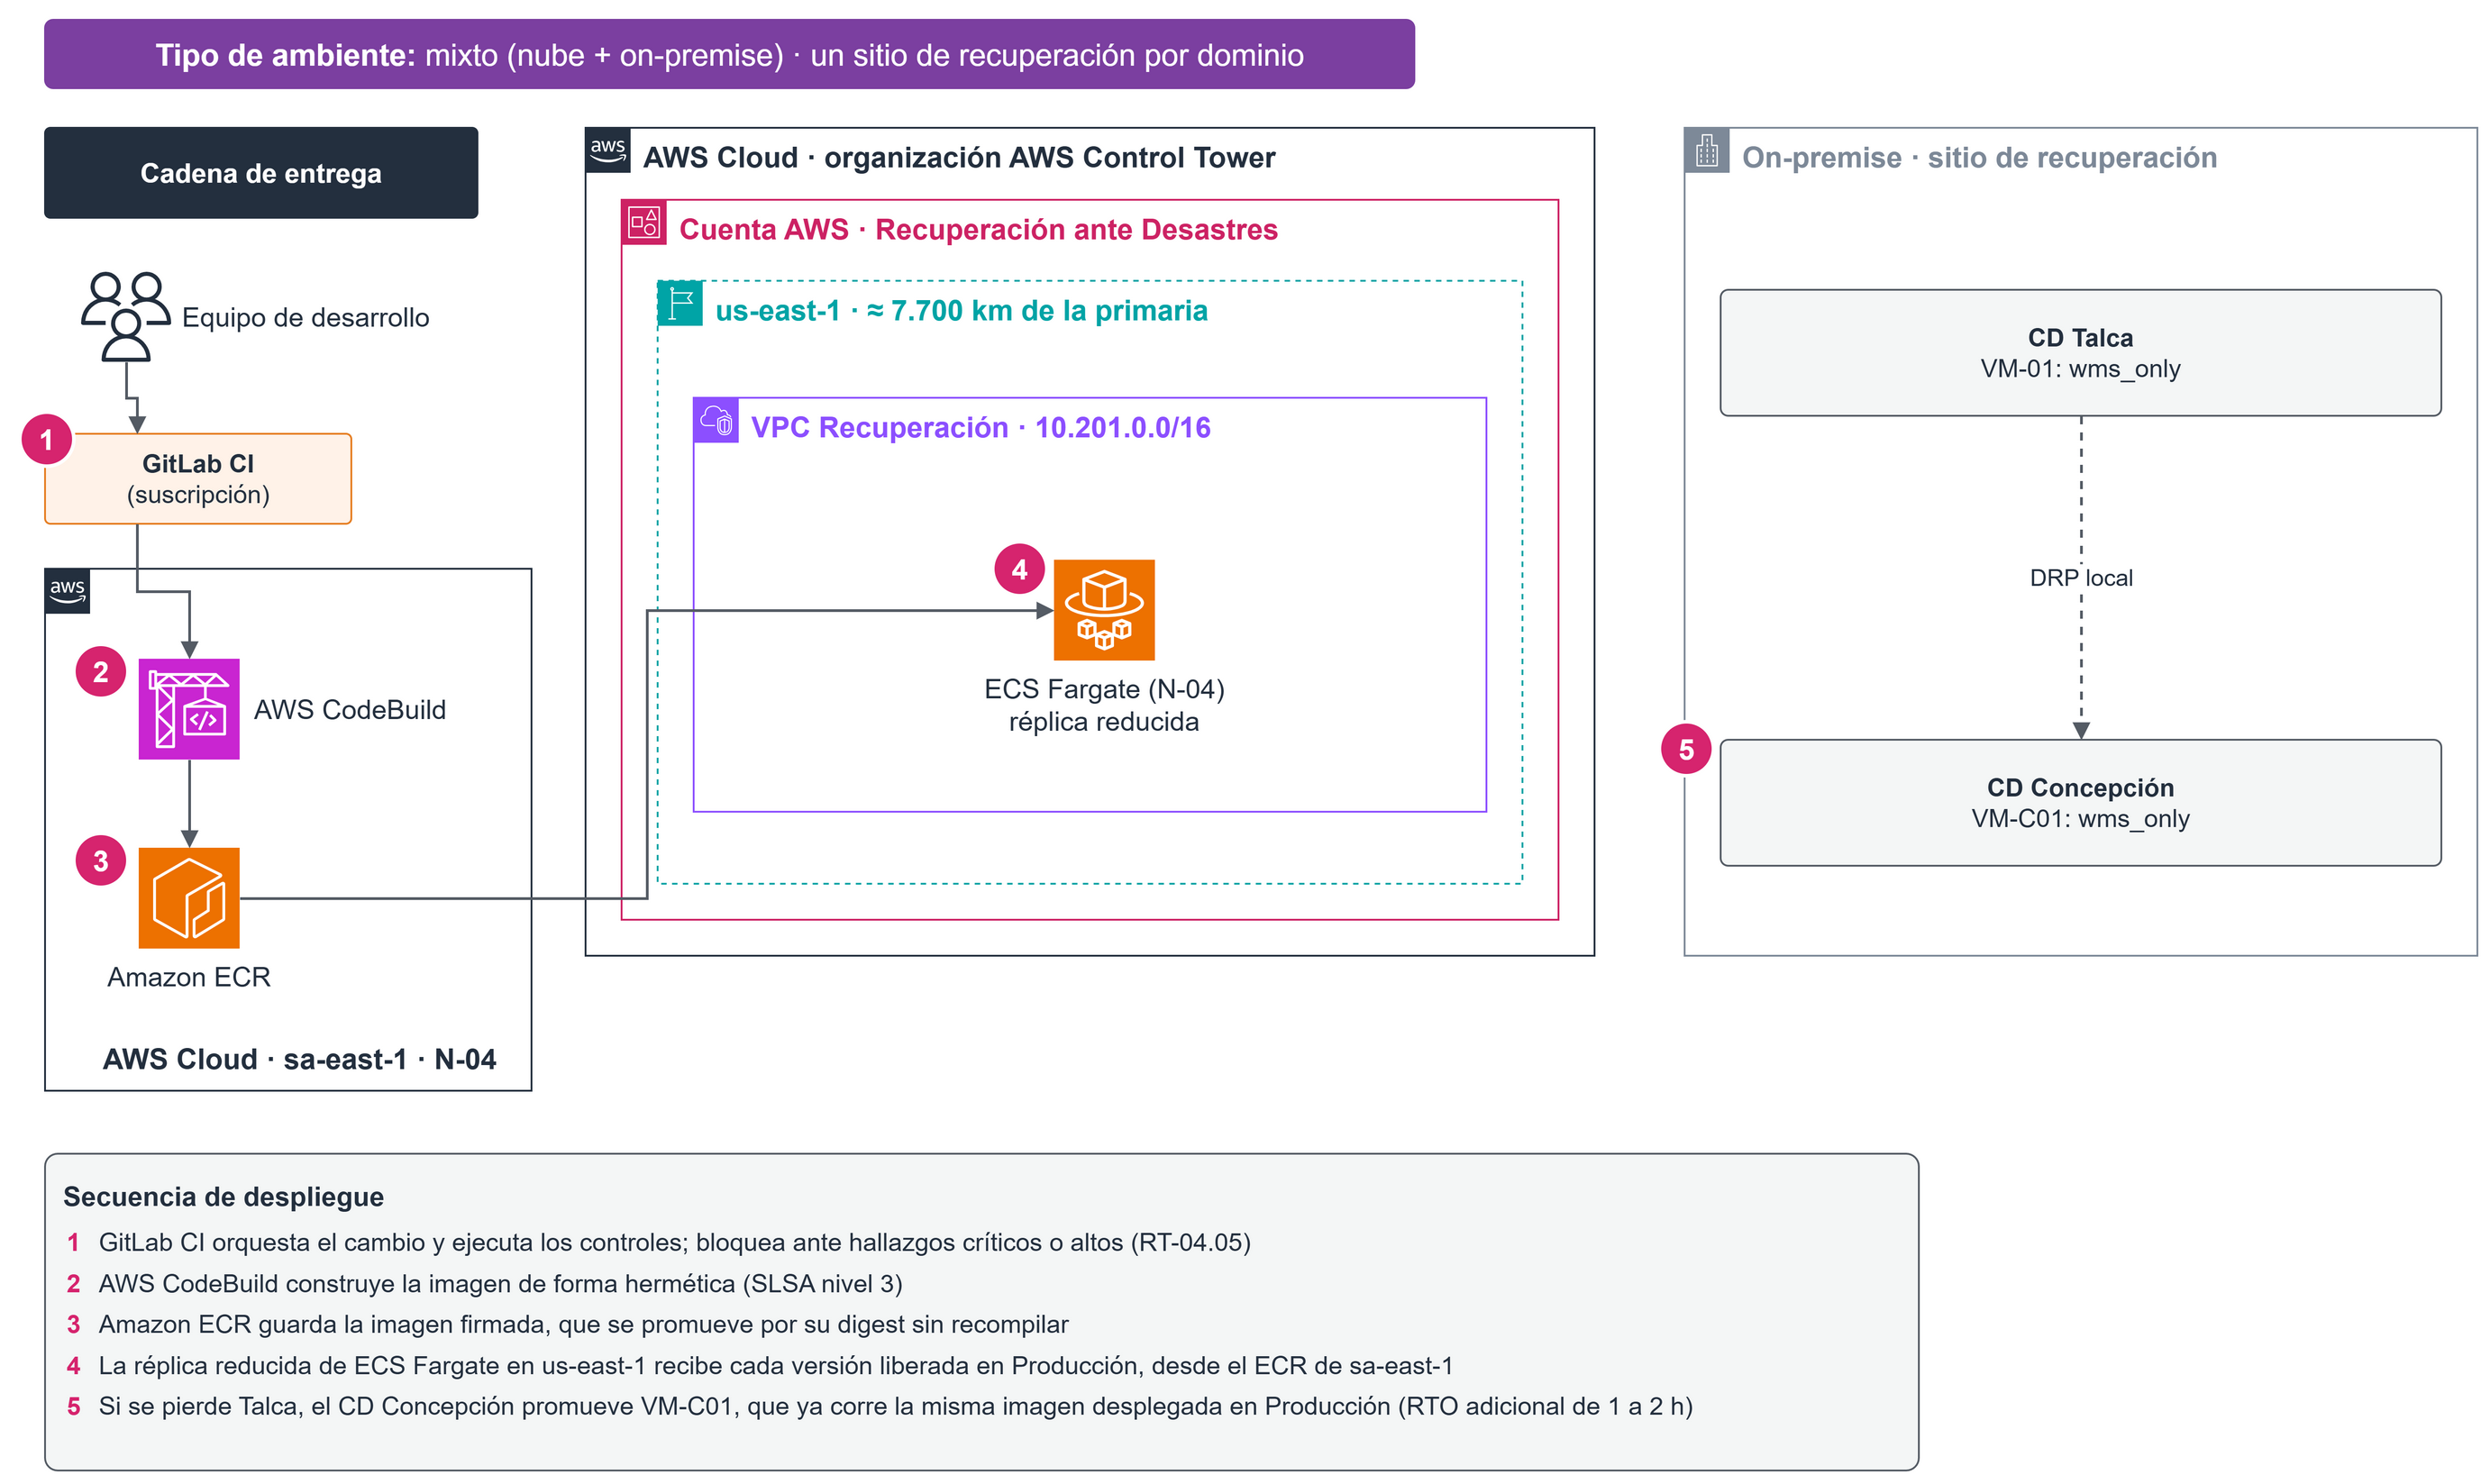
\includegraphics[width=\textwidth]{figuras/fisica/ambientes/amb_recuperacion.png}
  \caption{Ambiente de Recuperación ante Desastres}\label{fig:amb-recuperacion}
  \fuentefigura
\end{figure}

Los pasos de la figura son los siguientes:

\begin{enumerate}
  \item GitLab CI libera la entrega en Producción.
  \item CodeBuild no vuelve a construir: la imagen es la misma que se liberó en Producción.
  \item ECR guarda la imagen firmada en sa-east-1.
  \item ECR replica cada entrega liberada en Producción a us-east-1, y la réplica reducida de ECS Fargate la despliega en la VPC 10.201.0.0/16. Si se pierde la región primaria, esa réplica escala a carga completa en menos de 30 minutos.
  \item Si se pierde la sala de Talca, el perfil \texttt{wms\_only} de Talca se levanta en ECS Fargate de la VPC de Producción, sobre la copia del WMS de Talca que AWS DMS mantiene en Aurora PostgreSQL (N-05). El WMS recuperado conserva la identidad de Talca y atiende a los terminales de la bodega por la VPN.
\end{enumerate}

Concepción no depende de esta recuperación: sigue operando su propia bodega.

Las cinco figuras comparten la misma cadena de entrega y la misma imagen firmada, y difieren en la cuenta, el bloque de direccionamiento y el alcance hacia los sitios. Solo Producción llega a las bodegas por la VPC Hub, y Recuperación ante Desastres conserva preparada la réplica reducida de us-east-1 y la recuperación del WMS de Talca en la nube.

El paso de un ambiente a otro lo controla el pipeline de integración continua: GitLab CI lo orquesta y AWS CodeBuild construye cada imagen de forma hermética, con procedencia SLSA nivel 3. Cada cambio instala las dependencias exactamente como las fija \texttt{composer.lock} y pasa por estos controles (RT-04.05; Bases Técnicas Transversales, cap. 4, p. 10):

\begin{itemize}
  \item Auditoría de dependencias con \texttt{composer audit} y pruebas PHPUnit.
  \item Análisis estático con PHPStan y Larastan, y formato con Laravel Pint.
  \item Pruebas de contrato contra OpenAPI 3.1 y AsyncAPI 2.6.
  \item Escaneo de secretos y de imágenes de contenedor, y medición de cobertura.
\end{itemize}

El pipeline bloquea el despliegue ante un hallazgo crítico o alto, ante un contrato público roto sin nueva edición o ante una cobertura de la lógica de negocio inferior al 70 \% (RT-04.11; Bases Técnicas Transversales, cap. 4, p. 11). Además aplica la política corporativa de LafroX del Subdocumento 1 (sección 1.3.1): bloquea toda versión con cobertura de pruebas unitarias inferior al 80 \%. Son dos métricas distintas, medidas en la misma ejecución del pipeline, y una versión debe superar ambas. Primero, la imagen aprobada se firma, se publica en Elastic Container Registry y se promueve por su digest, de modo que ningún ambiente recompila. El paso a Producción es automático una vez que la imagen supera los controles del pipeline y el ensayo en Preproducción, dentro de las ventanas de la Tabla~\ref{tab:jd02} (RT-04.06; Bases Técnicas Transversales, cap. 4, p. 11). Segundo, la configuración no sensible se externaliza por ambiente en SSM Parameter Store y los secretos se gestionan en AWS Secrets Manager con rotación automática (ADR-15, Anexo 4-O). La imagen no contiene secretos ni el archivo de entorno (RT-04.08 y RT-04.09; Bases Técnicas Transversales, cap. 4, p. 11). Tercero, las migraciones de base de datos son migraciones Laravel basales y aditivas, que siguen la estrategia de expandir y contraer: se ejecutan como un paso único del despliegue antes de cambiar el tráfico, cada entrega solo agrega estructuras, de modo que la entrega previa y la nueva de la aplicación funcionan sobre el mismo esquema durante el despliegue, y las estructuras obsoletas se eliminan en una entrega posterior. Cada migración declara además su reversión, de modo que el esquema puede volver a la entrega previa (RT-04.10; Bases Técnicas Transversales, cap. 4, p. 11). Luego, el código reside en un repositorio con ramas protegidas, revisión obligatoria por pares y sin escritura directa sobre la rama principal (RT-04.03; Bases Técnicas Transversales, cap. 4, p. 10).

A Producción no se llega de otra forma: su acceso es restringido y auditado, y los desarrolladores no tienen acceso interactivo directo a ese ambiente (numeral 4.1 de las Bases Técnicas Transversales; Bases Técnicas Transversales, cap. 4, p. 10). El acceso privilegiado excepcional reúne estos controles:

\begin{itemize}
  \item IAM Identity Center federado con Keycloak por SAML 2.0 y SCIM, y MFA.
  \item Conjuntos de permisos temporales con aprobación previa y sesiones ECS Exec o Session Manager con registro de comandos y salida.
  \item SSH y el reenvío de puertos bloqueados.
\end{itemize}

La cuenta de último recurso (ADR-06, Anexo 4-O) se usa solo ante la indisponibilidad del IdP, con doble custodia, alerta inmediata, rotación de credenciales tras su uso y revisión posterior registrada.

Los portales de clientes, transportistas y proveedores siguen el mismo ciclo: su aplicación Angular se publica por ambiente en S3 privado y CloudFront, con la imagen de aplicación del mismo ambiente como backend. Las consolas Angular, en cambio, corren como contenedor en ECS Fargate tras el balanceador de aplicación privado (N-04).

\subsubsection{Artefacto y perfiles de ejecución}

El flujo de integración continua ejecuta automáticamente en QA las pruebas de carga de regresión, con el perfil versionado de 4-W.12, en cada versión candidata y al menos una vez por semana dentro del horario de uso del ambiente, y repite el ensayo en Preproducción antes de liberar. Compara percentil 95, errores y colas con la última versión aceptada bajo la misma carga y configuración; una regresión de desempeño o un incumplimiento de 4.2.6.11 bloquea la promoción hasta corregirla (RT-09.10; Bases Técnicas Transversales, cap. 9, p. 22).

La aplicación se construye una sola vez por entrega como una imagen PHP 8.5 con Laravel 13 que contiene el código, el \texttt{vendor} resuelto desde \texttt{composer.lock}, PHP-FPM, el intérprete de línea de comandos y las extensiones que la solución usa: \texttt{pdo\_pgsql}, \texttt{mbstring}, \texttt{intl}, \texttt{openssl}, \texttt{opcache}, \texttt{curl} para el SDK de AWS, \texttt{sockets} para el adaptador AMQP \texttt{php-amqplib}, la extensión de OpenTelemetry y \texttt{pcntl}, que solo usan los procesos de línea de comandos para terminar de forma ordenada al recibir la señal de detención. Un servidor web liviano acompaña a PHP-FPM en los perfiles HTTP. La misma imagen corre en todos los ambientes y en todos los sitios, y lo que cambia es el perfil con que arranca, como muestra la Tabla~\ref{tab:perfiles}. Cada perfil se despliega y revierte por separado, por lo que un componente crítico cambia de entrega sin detener a los demás (RT-02.02; Bases Técnicas Transversales, cap.~2, p.~6).

\begin{tablalafrox}{Perfiles de ejecución del artefacto Laravel}{tab:perfiles}%
  {F{0.20} Y F{0.24} F{0.18}}%
  {\cab{Perfil} & \cab{Proceso y función} & \cab{Dónde corre} & \cab{Escala por}}
  API & Servidor web y PHP-FPM con las APIs de M1--M12 para portales, preventa y reparto & N-04, ECS Fargate en 2 zonas & Procesos PHP-FPM ocupados sobre 70~\%, de 2 a 4 tareas y techo de 8 \\
  \texttt{wms\_only} & Servidor web y PHP-FPM con M1, M2, M5, la función local de bloqueo de M9 y la recepción física de retornos de M8, con la puerta de API local & VM-01, VM-C01 y E-01 & Fijo, dimensionado al sitio \\
  Shipper & PHP CLI que lee RabbitMQ con \texttt{php-amqplib}, publica sobres JSON en las colas FIFO de reconciliación y de solicitudes al ERP, fuera de Talca, recibe las respuestas de su sitio y lee la cola de coordinación de reservas de su sitio & VM-03, VM-C04 y E-01 & Uno activo por sitio \\
  Consumidor de reconciliación & PHP CLI con el SDK de AWS que aplica los sobres al estado central & N-04, ECS Fargate & Edad del mensaje más antiguo, de 2 a 4 tareas \\
  Trabajos & PHP CLI con el trabajador de colas de Laravel, con notificaciones y EDI en colas separadas & N-04, ECS Fargate & Profundidad de cada cola, de 2 a 4 tareas \\
  \texttt{erp-sync} & PHP CLI que consume RabbitMQ local y, por conexión saliente, la cola FIFO de solicitudes al ERP, y emite mediante A-04 & VM-04, Talca & Dos procesos fijos \\
  Planificador & PHP CLI para las tareas periódicas del ambiente & N-04, una sola tarea por ambiente & No escala \\
\end{tablalafrox}

{\footnotesize Fuente: elaboración propia.\par}

Los perfiles comparten la revisión de código y el esquema de datos, pero cada uno tiene su propio rol de IAM o credencial local, con solo los permisos que su función necesita: el perfil de API no puede leer la cola de reconciliación, el consumidor no puede escribir en las colas de trabajos, el shipper solo puede enviar a las colas de reconciliación y de solicitudes al ERP y leer la respuesta y la coordinación de reservas de su sitio, y \texttt{erp-sync} es el único lector de las solicitudes al ERP. El planificador corre como una sola tarea por ambiente, con despliegue que detiene la tarea en ejecución antes de iniciar la nueva, y cada tarea periódica toma además un bloqueo en la base de datos para impedir ejecuciones superpuestas. Los sitios no ejecutan planificador: sus procesos permanentes son el servidor del WMS y el shipper, además de \texttt{erp-sync} en VM-04 de Talca. En los centros de distribución, el perfil \texttt{wms\_only}, que es el Motor WMS A-01, corre como contenedor en VM-01 y VM-C01, y el shipper corre junto al broker de colas A-03, RabbitMQ, en VM-03 y VM-C04, todos sobre las máquinas virtuales de Proxmox. En cada cross-docking, el perfil \texttt{wms\_only} y el shipper se orquestan con Docker Compose en E-01, junto a PostgreSQL, RabbitMQ y la caché de identidad. En Concepción y en cada cross-docking, el equipo en espera mantiene detenidos el WMS y el shipper; solo ejecuta la réplica de PostgreSQL, la caché de identidad y el colector de observabilidad hasta que toma el control. Los sitios descargan la imagen desde Elastic Container Registry por la VPN, a través de la VPC Hub, y los endpoints de interfaz de la VPC de Producción, en conexiones salientes y sin tráfico por Internet. Ansible (F-02), con el que se declara como código la configuración de los cinco sitios, actualiza sus contenedores sitio por sitio. Elastic Container Registry replica cada imagen liberada de sa-east-1 a us-east-1 mediante replicación entre regiones, de modo que la réplica reducida y la plataforma promovida en una conmutación usan el mismo digest sin depender del registro primario. En us-east-1, la infraestructura como código deja creadas y vacías las colas SQS FIFO y SQS, y los temas SNS equivalentes, a las que se redirigen los shippers y \texttt{erp-sync} durante la conmutación. Fuera de la imagen Laravel quedan el frontend Angular de las consolas, el motor de rutas M4 y el transporte AS2 M11, los tres en contenedores propios sobre ECS Fargate (N-04) y construidos por el mismo pipeline. M11 opera tras contratos versionados (ADR-11, Anexo 4-O).

El transporte AS2 y el frontend de consolas mantienen dos tareas cada uno, distribuidas entre dos zonas de disponibilidad (RT-03.02; Bases Técnicas Transversales, cap. 3, p. 8). El motor de rutas ejecuta una tarea por corrida. Si falla, ECS la relanza en otra zona y repite la corrida dentro de la planificación de 15:00 a 18:30, y la prueba de aceptación mide el plazo de 20 min por corrida.

Cada perfil cumple este ciclo de vida:

\begin{enumerate}
  \item Arranque y compatibilidad de esquema: el contenedor verifica la edición esperada y no acepta tráfico ni mensajes si no coincide.
  \item Comprobación de salud: los perfiles HTTP exponen una ruta de salud de proceso, que usa el balanceador, y otra de disponibilidad que comprueba la base y la cola. Los procesos de línea de comandos informan su salud por un latido que vigila el orquestador.
  \item Detención y drenaje: el balanceador deja de enviar solicitudes nuevas y espera 30 segundos a que terminen las vigentes. Los trabajadores reciben la señal de detención, terminan el mensaje en curso sin tomar otro y salen antes de 120 segundos, plazo mayor que el tiempo máximo de un trabajo. El mensaje no confirmado vuelve a la cola al vencer su visibilidad.
\end{enumerate}

Así, ningún reinicio, escalado o despliegue deja un trabajo a medias.

\subsubsection{Liberación y reversión}

Cada entrega se libera con estrategia azul-verde: la entrega nueva se despliega junto a la vigente y recibe tráfico de forma gradual, en etapas de canario, después de haberse demostrado el mismo procedimiento en Preproducción (RT-04.07; Bases Técnicas Transversales, cap. 4, p. 11). La puesta en producción avanza por proceso, por sitio o por zona comercial, nunca como un evento único que afecte a la vez a la bodega, la preventa, el reparto y la facturación. En la sustitución del WMS de 2013 por olas, cada capacidad se activa además por sitio mediante indicadores de funcionalidad (\emph{feature flags}), sin volver a desplegar. Revertir una ola devuelve el tráfico a la entrega previa del nuevo servicio. El WMS de 2013 ya no escribe stock y se retira al cerrar la marcha blanca de Talca.

Mientras dura el canario, la entrega previa permanece desplegada, por lo que revertir es devolverle el tráfico, sin recompilar ni volver a desplegar. La reversión es automática y se dispara cuando el percentil 95 de una transacción supera su umbral comprometido (Tabla~\ref{tab:t84}) o cuando la entrega nueva registra más errores que la estable en la misma ventana de observación. No se pierde ninguna transacción confirmada: las operaciones en curso quedan en los buffers locales, 24 horas por sitio en el broker y la caché de turno en los dispositivos, y se reprocesan de forma idempotente contra la entrega restituida. El esquema no necesita revertirse durante el canario, porque la migración de la entrega solo agregó estructuras. Si hiciera falta, la reversión declarada de la migración lo devuelve a la entrega previa. La reversión cambia la imagen en servicio sin perder operaciones. El tiempo efectivo de reversión tiene un objetivo $\leq$ 10 minutos, medido en cada ensayo en Preproducción. El tiempo medio de restauración de incidentes críticos $\leq$ 4 horas es una métrica mensual de operación distinta de la reversión técnica (Bases Administrativas, art. 78.3, p. 40).

Si la falla de un despliegue se manifestara durante la ventana de despacho, la bodega y el reparto continuarían con su operación local (Tabla~\ref{tab:t29}) mientras se revierte, sin detener la salida de los camiones.

Cada promoción ensaya además la compatibilidad de los mensajes retenidos. Un sitio puede volver de un corte de 24 horas con sobres publicados por la entrega previa, de modo que el consumidor de reconciliación acepta la edición vigente y la inmediatamente previa del sobre JSON, y rechaza hacia la cola de mensajes fallidos cualquier edición que no reconozca, sin aplicarla. Preproducción reproduce ese caso ---sitio emulado desconectado, promoción de la entrega nueva y reconexión--- antes de cada paso a producción.

\subsubsection{Implantación por olas en los sitios}

La arquitectura lógica fija la implantación progresiva por olas (apartado 4.1.8). Su secuencia física es la siguiente:

\begin{enumerate}
  \item Se registran los contratos OpenAPI y AsyncAPI, el sobre JSON, el esquema PostgreSQL de destino definido por el modelo de datos de la solución, que es la línea base de las migraciones Laravel, y el extracto conciliado del WMS de 2013 de Talca.
  \item Se construye el backend y se prueban las colas y la capa anticorrupción con fallas inducidas: corte de enlace, ERP caído, mensajes duplicados y fuera de orden.
  \item Se habilita un sitio piloto, dimensionado por su capacidad real, y el WMS de 2013 deja de escribir cada capacidad que se migra. El tráfico se migra por olas con un único escritor autorizado para cada operación. Nunca escriben a la vez el WMS de 2013 y la solución sobre el stock, los cobros o los documentos tributarios.
  \item Antes de cada corte se drenan o se transforman al sobre JSON vigente los mensajes de ediciones anteriores del propio sobre que el consumidor no admita.
  \item Cada ola cierra verificando saldos de stock, cobros y folios contra el extracto del origen, y se revierte por sitio si falla un umbral acordado con el CLIENTE.
  \item La reversión devuelve el tráfico a la entrega previa del nuevo servicio solo después de detener la nueva, conciliar los mensajes retenidos y comprobar que el esquema sigue legible por la entrega previa. No reactiva el WMS de 2013 como escritor.
\end{enumerate}

\subsubsection{Calendario y cadencia}

El calendario de Puelche limita cuándo se puede intervenir la plataforma. El caso prohíbe intervenir los sistemas entre el 1 y el 25 de septiembre, en diciembre y durante el cierre contable de cada mes, prohíbe el paso a producción en todo septiembre y en diciembre, y exige indisponibilidad cero en la ventana de despacho (Bases Técnicas del caso, cap. 10, restricción 8, p. 19, y Cap. 13, p. 23; RT-10.05 y RT-10.06; Bases Técnicas Transversales, cap. 10, p. 22; Bases Técnicas del caso, cap. 15, p. 27). La Tabla~\ref{tab:jd02} cruza cada período con lo que admite.

\begin{tablalafrox}{Ventanas de despliegue}{tab:jd02}%
  {F{0.36} F{0.26} Y}%
  {\cab{Período} & \cab{Despliegue} & \cab{Indisponibilidad programada}}
  Todo septiembre, sin intervención alguna del 1 al 25 & No & No \\
  Todo diciembre & No & No \\
  Tres primeros días hábiles del mes & No & No \\
  05:30--07:00, lunes a sábado & No & No \\
  22:00--06:00, preparación de pedidos & Sí, sin interrupción & No \\
  08:00--18:00, recepción de proveedores & Sí, sin interrupción & No \\
  Resto del calendario & Sí, sin interrupción & Excepcional, con aviso de 10 días hábiles \\
\end{tablalafrox}

{\footnotesize Fuente: elaboración propia a partir de las Bases Técnicas del caso (cap. 10, p. 19).\par}

El despliegue sin interrupción es, por lo tanto, la regla y no una capacidad opcional: solo fuera de las ventanas protegidas se admite una indisponibilidad programada, y únicamente por excepción. En la ventana nocturna, además, toda intervención en bodega considera el turno de preparación. Descontados los congelamientos, quedan unos diez meses desplegables al año, de los que se excluyen los tres primeros días hábiles de cada mes. Sobre ese margen se fija una cadencia quincenal de despliegue y un tiempo de hasta cinco días hábiles desde que se confirma un cambio de código hasta que llega a producción, compatible con el plazo de siete días corridos para remediar una vulnerabilidad crítica (Artículo 21.1 de las Bases Administrativas (art. 21.1, p. 15); RT-11.04; Bases Técnicas Transversales, cap. 11, p. 23). La tasa de cambios fallidos no supera el 5 \% de los despliegues del mes y el tiempo de restauración no supera 4 horas, conforme al Artículo 78.3 de las Bases Administrativas (art. 78.3, p. 40). Estas cuatro métricas se miden durante la Operación (RT-04.12; Bases Técnicas Transversales, cap. 4, p. 11). Las correcciones de incidentes críticos usan el mismo pipeline, con prioridad y fuera de la cadencia quincenal, dentro del plazo de resolución de 4 horas. Cada servicio crítico tiene como presupuesto de error el complemento de su disponibilidad comprometida de 99,9~\% mensual, unos 43 minutos al mes. Si un servicio lo consume, se suspenden en él los despliegues que no sean correctivos hasta el mes siguiente (RT-10.09; Bases Técnicas Transversales, cap. 10, p. 22).

\subsection{Red de despliegue}
\label{sub:2-redes-topologia-segmentacion-y-conectivi}

La sección de conexiones describe los caminos entre los sitios, el terreno y la nube, y su conmutación (Tabla~\ref{tab:conexiones}). El despliegue agrega tres definiciones sobre esa red: dónde llegan los túneles, cómo se reparte el direccionamiento y cómo se dirige el tráfico entre regiones.

Los túneles de AWS Site-to-Site VPN de los cinco sitios llegan a la VPC Hub de sa-east-1, donde el Transit Gateway los une solo a la VPC de Producción. La región us-east-1 dispone de su propio Transit Gateway y de su VPN para reconectar los sitios durante una conmutación. La de Producción es la única VPC con enlace hacia los sitios, coherente con que el on-premise es producción: Desarrollo, QA y Preproducción no tienen conectividad con las bodegas, de modo que un error en un ambiente de prueba no puede alcanzarlas. El direccionamiento se asigna sin solapamiento, según la Tabla~\ref{tab:t64}, y el bloque de recuperación 10.201.0.0/16 corresponde al ambiente de Recuperación ante Desastres de la Tabla~\ref{tab:t62}.

\begin{tablalafrox}{Direccionamiento y segmentación}{tab:t64}%
  {F{0.30} F{0.27} Y}%
  {\cab{Dominio} & \cab{Bloque} & \cab{Segmentación}}
  Talca & 10.1.0.0/16 & VLAN de gestión, servidores, operación, estaciones e IoT \\
  Concepción & 10.2.0.0/16 & Mismas VLAN que Talca \\
  Cross-docking & 10.3.0.0/16 a 10.5.0.0/16 & VLAN de gestión y de operación tras el par de firewalls del sitio, por la VPN \\
  Sitios adicionales previstos & 10.6.0.0/16 y 10.7.0.0/16 & Reservados \\
  VPC Hub de conectividad, sa-east-1 & 10.100.0.0/16 & Transit Gateway y terminación VPN de los cinco sitios \\
  VPC Producción, zona pública & 10.101.1.0/24 y 10.101.2.0/24 & NAT y Network Load Balancer del canal AS2 \\
  VPC Producción, zona privada & Resto de 10.101.0.0/16 & ALB de aplicación y consolas, aplicación y datos, enlazada a los sitios por el Transit Gateway de la VPC Hub \\
\end{tablalafrox}

{\footnotesize Fuente: elaboración propia.\par}

Cada sitio con cómputo dispone de un bloque propio. La séptima instalación que el caso proyecta a tres años y el centro de distribución que Puelche evalúa abrir hacia 2030 en la Región de Los Lagos tienen reservados 10.6.0.0/16 y 10.7.0.0/16, de modo que su incorporación es una parametrización de la infraestructura como código (RT-02.12; Bases Técnicas Transversales, cap. 2, p. 7; Bases Técnicas del caso, cap. 15, p. 26). En la nube, los ALB de aplicación y consolas son privados, y la subred pública solo aloja NAT y el Network Load Balancer del canal AS2. Los portales residen en S3 privado, servido únicamente por CloudFront. La VPC de Producción usa endpoints de interfaz execute-api, IoT Core, SQS, SSM y Elastic Container Registry, y endpoints de puerta de enlace para DynamoDB y S3. Como los de puerta de enlace no son alcanzables desde los sitios por la VPN, los sitios descargan la imagen por el endpoint de interfaz de Elastic Container Registry y por un endpoint de interfaz de S3, donde se almacenan las capas de las imágenes, sin salir a Internet.

El tráfico externo sigue las entradas de la sección~\ref{sub:superficie}. Route 53 cambia el tráfico regional después de la autorización del CLIENTE, la promoción de Aurora, la restitución de la identidad, las API pública y privada y Verified Access, y la validación funcional. Luego se reconectan la VPN y los brokers (Tabla~\ref{tab:4-3-6}).

La red también debe devolver a la normalidad a un sitio que operó desconectado. El compromiso es resincronizar la flota en hasta 10 minutos y un centro de distribución en hasta 2 horas después de un corte de 24 horas (Tabla~\ref{tab:t29}). Un corte de 24 horas acumula los cambios de la base con su registro de escritura anticipada, el vaciado del broker, la telemetría, la observabilidad y el incremental de respaldo: unos 1,68 GB en Talca, 1,29 GB en Concepción y 0,32 GB en cada cross-docking, que se drenan en 2 horas con 1,87, 1,44 y 0,35 Mbps, respectivamente (Tabla~\ref{tab:t81}; Anexo 4-W). La evidencia de entrega no se suma al drenaje, porque durante el corte del centro de distribución el terminal la envía por la red celular. Las reservas de capacidad y la prioridad de cada camino se detallan en la Tabla de ancho de banda de 4.2.6. La operación de bodega conserva su autonomía mientras se drenan los mensajes. Al reconectar, la calidad de servicio prioriza el broker y el registro de escritura anticipada sobre la telemetría.

\subsection{Alta disponibilidad}
\label{sub:3-alta-disponibilidad}

No todos los servicios necesitan el mismo nivel de continuidad. El Artículo 78 (Bases Administrativas, art. 78.2, p. 40) fija cuatro niveles de servicio, y la solución asigna cada servicio a uno según el efecto de su indisponibilidad sobre la operación (RT-10.02; Bases Técnicas Transversales, cap. 10, p. 22), como muestra la Tabla~\ref{tab:jd05}.

\begin{tablalafrox}{Clasificación de servicios por nivel de servicio}{tab:jd05}%
  {F{0.12} H{0.18} H{0.14} Y}%
  {\cab{Nivel} & \cab{Disponibilidad} & \cab{Resolución} & \cab{Servicios}}
  Crítico & 99,9 \% & 4 h & Preparación y despacho con emisión de la guía requerida por un cambio de carga en la ventana de 05:30 a 07:00, con el bloqueo por excursión térmica y la identidad de bodega que lo habilitan \\
  Alto & 99,5 \% & 8 h & Toma de pedido de preventa y consulta de stock y crédito, entrega y evidencia de entrega, planificación de rutas, otros documentos tributarios, integración con el ERP, cobranza y rendición, y registro de temperatura \\
  Medio & 99,0 \% & 24 h & Canal moderno (EDI), notificaciones, analítica y tableros, portales, consultas de geolocalización y registros de auditoría y seguridad \\
  Bajo & 98,0 \% & 48 h & Reportería e informes a pedido \\
\end{tablalafrox}

{\footnotesize Fuente: elaboración propia a partir de las Bases Administrativas (art. 78.2, p. 40).\par}

El plazo de 4 h de la guía nueva supone el ERP disponible. Si se pierde la sala de Talca, la guía nueva espera que el CLIENTE restituya el servidor del ERP. Mientras tanto, solo sale la carga amparada por su guía preemitida (sección~\ref{sub:conmutacion-regional}).

Las clases de servicio se distinguen por su alternativa operativa:

\begin{itemize}
  \item Crítico: detiene un proceso sin alternativa. La ventana de despacho de 05:30 a 07:00 no admite ejecución manual, la nueva guía por un cambio de carga se emite antes de salir y el bloqueo por excursión térmica y la identidad de bodega condicionan la salida.
  \item Alto: tiene una alternativa costosa. La toma de pedido, la entrega y la consulta de stock y crédito siguen siendo transacciones críticas en desempeño (Tabla~\ref{tab:t84}), pero el dispositivo las captura sin conexión durante un turno completo y las sincroniza al reconectar. La ruta puede planificarse a mano en 3,5 horas y las transacciones hacia el ERP distintas de la guía de la ventana de despacho se retienen en cola hasta 24 horas.
  \item Medio: dispone de una alternativa operativa.
  \item Bajo: no impide operar.
\end{itemize}

El compromiso penalizable del 99,9 \% recae sobre la preparación y el despacho, que se ejecutan contra la base local del centro de distribución sin atravesar la WAN, y sobre la identidad, cuya autoridad reside en la nube y se sostiene con el despliegue en varias zonas de disponibilidad (apartado 4.3.1.2).

Esa es la razón por la que el 99,9 \% de extremo a extremo no depende de multiplicar las disponibilidades de la infraestructura. El numeral 7.2 de las Bases Técnicas Transversales (cap. 7, p. 17) fija un mínimo de 99,95 \% mensual para la energía, la climatización, la red, el cómputo, la base de datos y los portales, pero esos valores son pisos por subsistema y su producto en serie quedaría por debajo del 99,9 \%. El compromiso se sostiene en la redundancia interna de cada subsistema y en la ruta que sigue cada transacción. La confirmación de preparación, la más estricta, se ejecuta contra la base local del centro de distribución y no atraviesa la WAN ni la nube. Descansa sobre energía y climatización en N+1, un par de firewall en alta disponibilidad, dos switches en stack, un clúster de tres nodos N+1 y almacenamiento Ceph con tres réplicas en NVMe sin RAID, con un solo elemento en serie, la instancia de escritura VM-02, que se reinicia en otro nodo del clúster (Tabla~\ref{tab:fallas-sitios}). La identidad, por su parte, se sostiene en la nube con Keycloak (A-05) en dos zonas y, en cada sitio, con la caché de solo lectura y el verificador local de relevo de turno.

En Concepción y en cada cross-docking, la misma confirmación se ejecuta en un par de equipos idénticos, uno activo y otro en espera, conforme a RT-03.14 (Bases Técnicas Transversales, cap. 3, p. 9). Concepción usa dos servidores Proxmox independientes: el activo ejecuta VM-C01 a VM-C04 y el otro, sus copias. Cada cross-docking usa dos mini-PC E-01. El mecanismo es el mismo en los cuatro sitios:

\begin{itemize}
  \item PostgreSQL del equipo activo replica cada transacción en forma sincrónica al de espera, de modo que una transacción confirmada existe en los dos equipos.
  \item Si el activo falla, el de espera promueve su base y toma la dirección virtual del sitio con keepalived (VRRP). Los terminales siguen trabajando contra la misma dirección y el sitio vuelve a operar en menos de un minuto.
  \item Para que no haya dos equipos activos, el de espera se promueve solo si deja de ver al activo por sus dos interfaces, conectadas a switches distintos.
  \item Al tomar el control, el equipo vuelve a publicar desde el outbox replicado los eventos de las últimas 24 horas, y la nube descarta por UUID los que ya recibió.
  \item Si falla el equipo en espera, la replicación pasa a asíncrona y se genera una alerta, para que el activo no se detenga. El equipo dañado se repone y se resincroniza desde el activo.
\end{itemize}

Solo la pérdida simultánea de los dos equipos obliga a reconstruir la base del sitio desde el estado central (Tabla~\ref{tab:fallas-sitios}).

En la nube, todos los servicios con requisito de alta disponibilidad operan en al menos dos zonas (RT-03.02; Bases Técnicas Transversales, cap. 3, p. 8):

\begin{itemize}
  \item Aurora PostgreSQL (N-05) escribe en sa-east-1a y mantiene un lector promovible en sa-east-1b, al que conmuta en menos de 30 segundos.
  \item ElastiCache mantiene primario y réplica entre esas zonas y conmuta en menos de 60 segundos.
  \item Las tareas de ECS Fargate se distribuyen en ambas zonas y se reprograman solas ante la pérdida de una.
  \item DynamoDB, el balanceador y los NAT Gateway son multizona por diseño.
\end{itemize}

Estos tiempos corresponden a los que AWS declara como habituales para cada servicio y se tratan como objetivos que se miden en las pruebas de la sección~\ref{sub:6-verificacion-de-la-continuidad}. Ante el peak de septiembre, el escalamiento automático y la degradación controlada del apartado de dimensionamiento sostienen los umbrales de desempeño sin intervención.

\subsection{Recuperación ante desastres}
\label{sub:4-recuperacion-ante-desastres-ba-art-20-rt}

La recuperación ante desastres es activo-pasiva en caliente: la región us-east-1 mantiene una réplica reducida pero funcional de la plataforma, escalable a carga completa en menos de 30 minutos, que se promueve solo cuando se pierde la región primaria. Los objetivos son un RTO de hasta 4 horas y un RPO de hasta 15 minutos para los servicios críticos (RT-07.04; Bases Técnicas Transversales, cap. 7, p. 17). Cada dominio de datos alcanza ese RPO con su propio mecanismo de replicación (Tabla~\ref{tab:4-3-4}): Aurora Global Database mantiene en us-east-1 la réplica promovible de la base en nube, DynamoDB Global Tables la telemetría, y la replicación de S3 entre regiones lleva la evidencia, los documentos y las copias de AWS Backup (N-11).

Si Talca pierde fibra y LTE, Starlink D-06, mantenido en espera caliente con el túnel IPsec establecido y BGP de menor preferencia, sostiene la lectura continua de AWS DMS sobre VM-02 y el envío de eventos críticos. La operación local conserva al menos 24 horas de autonomía. El límite residual del RPO y sus mitigaciones se exponen en 4.3.2, bajo «RPO y RTO». El registro retenido se acota con un tope de 5 GB por slot, frente a los unos 0,123 GB diarios de registro de escritura anticipada que estima el dimensionamiento para Talca: cubre con amplio margen un corte de 24 horas y ocupa como máximo la cuarta parte de los 20 GB actuales de VM-02, que crecen a 31 GB a 3$\times$, sin arriesgarlo (Anexo 4-W). El retraso de replicación y el tamaño del registro retenido se miden de forma continua y generan alarma a los 5 y a los 15 minutos de retraso.

La réplica por DMS y la reconciliación por eventos cumplen funciones distintas y no se mezclan. DMS copia las tablas del WMS de Talca (VM-02) a un esquema de réplica de solo lectura en Aurora, que sirve a la continuidad y a las consultas. Concepción y los cross-docking no replican sus bases por DMS: publican sus eventos mediante los brokers y SQS FIFO. El consumidor de reconciliación aplica esos sobres JSON a las tablas de dominio del estado central ---stock consolidado, trazabilidad de lotes, pedidos, entregas y cobros---, y en la misma transacción registra la clave de origen del evento, formada por el sitio y el identificador único que el evento trae desde su captura. Una restricción de unicidad sobre esa clave impide aplicar dos veces el mismo evento, aunque SQS lo entregue de nuevo o llegue después de la ventana de deduplicación de la cola. Ninguna tabla de dominio se alimenta de la réplica DMS, y ningún evento escribe en el esquema de réplica.

\subsubsection{Conmutación y retorno}

La conmutación de región y el retorno siguen el procedimiento de la sección~\ref{sub:conmutacion-regional} (Tabla~\ref{tab:4-3-6}): la promoción de la base exige la autorización del CLIENTE y el enrutamiento hacia us-east-1 cambia después de la validación funcional. El retorno se ejecuta de forma coordinada tras la reconciliación. Si la contingencia afecta solo a la sala de Talca, su WMS se levanta en Fargate sobre su copia en Aurora de la región activa. Los dominios de recuperación y sus amenazas comunes se analizan en la Tabla~\ref{tab:4-3-3}.

\subsubsection{Operación durante una contingencia regional}

Mientras la región primaria no está disponible, la bodega y el terreno siguen operando contra sus bases locales y sus dispositivos. Tras la autorización del CLIENTE, la plataforma se promueve en us-east-1 y recupera las transacciones en nube. La analítica se recupera después desde su copia diferida, y las consultas de geolocalización de personas, excluidas de us-east-1 por diseño (sección~\ref{sec:e-especificaciones-del-sitio-secundario-y-}), esperan el retorno. Ninguna es un servicio crítico.

\subsection{Respaldos}
\label{sub:5-respaldos-esquema-3-2-1-1-0-rnf-20-07}

El respaldo protege contra lo que las réplicas replican: un dato borrado por error, corrompido o cifrado de forma maliciosa. La solución aplica el esquema 3-2-1-1-0 exigido para la nube y el on-premise, con una copia inmutable (RT-07.09; Bases Técnicas Transversales, cap. 7, p. 18). Mantiene tres copias en dos medios, base de datos y almacenamiento de objetos:

\begin{itemize}
  \item Los datos activos.
  \item Una segunda copia, formada por las instantáneas de Aurora y, para el WMS de Talca, por la copia local D-05.
  \item El respaldo exportado a S3.
\end{itemize}

Una copia está fuera del sitio, replicada a us-east-1 por AWS Backup (N-11) y la replicación de S3, y otra es inmutable, en S3 Object Lock en modo Compliance con AWS Backup Vault Lock. El cero corresponde a los errores de verificación de restauración: cada mes se restaura una muestra rotativa que recorre todos los dominios de la Tabla~\ref{tab:jd12}, se mide el tiempo efectivo de restauración y todo error se corrige antes de la verificación siguiente (RT-07.12; Bases Técnicas Transversales, cap. 7, p. 18).

La copia inmutable es el control frente a un ataque con credenciales administrativas comprometidas: en modo Compliance, ni un administrador ni la cuenta raíz pueden borrarla ni modificarla durante su retención, y el bloqueo de la bóveda, con 3 días de enfriamiento y una retención mínima de 35 días, igual a la menor retención de la Tabla~\ref{tab:jd12}, impide eliminar los respaldos una vez activado (RT-07.11; Bases Técnicas Transversales, cap. 7, p. 18). La copia local D-05 cumple otra función: es la copia de recuperación rápida, cifrada con una clave independiente de la de producción, que permite restaurar el WMS en hasta 4 horas sin depender del enlace, y por eso no se cuenta como la copia inmutable. Un medio físico cifrado se rota además cada semana a una bóveda externa, y se conserva en el recinto de custodia declarado en el Formulario T-11 hasta su traslado.

La Tabla~\ref{tab:jd12} muestra, para cada dominio de datos, con qué frecuencia se respalda, cuánto tiempo se retiene y en cuánto tiempo se restaura por completo (RT-07.13; Bases Técnicas Transversales, cap. 7, p. 18).

\begin{tablalafrox}{Respaldo y restauración por dominio de datos}{tab:jd12}%
  {Y F{0.30} H{0.16} H{0.17}}%
  {\cab{Dominio} & \cab{Frecuencia} & \cab{Retención} & \cab{Restauración}}
  Transaccional de bodega & Continua, con copia local D-05 en Talca y, en Concepción y los cross-docking, reconstrucción desde el estado central & 35 días & $\leq$ 4 h \\
  Transaccional en nube & Diaria y recuperación continua & 35 días & $\leq$ 4 h \\
  Identidad & Diaria y recuperación continua & 35 días & $\leq$ 4 h \\
  Trazabilidad sanitaria & Continua & Vida útil + 6 meses, mínimo 5 años & $<$ 2 h \\
  Registros de temperatura & Diaria y continua & 5 años & $\leq$ 8 h \\
  Evidencia de entrega & Continua con versionado & 6 años & $\leq$ 8 h \\
  Respaldo de documentos tributarios & Continua con versionado & 6 años & $\leq$ 8 h \\
  Geolocalización de personas & Continua & 12 meses & $\leq$ 24 h \\
  Registros de seguridad y auditoría & Continua & 7 años & $\leq$ 24 h \\
\end{tablalafrox}

{\footnotesize Fuente: elaboración propia.\par}

Cada tiempo de restauración corresponde al plazo de resolución que el Artículo 78.2 de las Bases Administrativas (art. 78.2, p. 40) asigna al servicio más crítico que usa el dato: la base transaccional en nube se restaura en 4 horas porque sostiene también la identidad, que es crítica, porque Keycloak guarda en Aurora sus datos (ADR-06, Anexo 4-O). La trazabilidad sanitaria es la única excepción más exigente: se restaura en menos de 2 horas, porque ese es el plazo en que Puelche debe responder un retiro sanitario (Bases Técnicas del caso, cap. 18, p. 34). Las retenciones cumplen o superan las del caso. La restauración, además, puede ser parcial: la recuperación de Aurora a un instante específico, sobre una instancia temporal, permite restituir un registro, una tabla, un módulo o el sistema completo sin intervenir el ambiente productivo (RT-07.14; Bases Técnicas Transversales, cap. 7, p. 18).

AWS Backup aplica a Aurora y DynamoDB los respaldos y la recuperación a un instante específico, mientras S3 aporta versionado, Object Lock y réplica entre regiones para los documentos legales. Object Lock protege también los registros de seguridad y auditoría. Los plazos y las retenciones por dominio constan en la Tabla~\ref{tab:jd12}.

\subsection{Verificación de la continuidad}
\label{sub:6-verificacion-de-la-continuidad}

Los mecanismos descritos se verifican con pruebas periódicas. Antes de cada paso a producción, y al menos una vez por semestre durante la Operación, se inyectan la caída de una instancia, de una zona, del equipo activo de Concepción o de un cross-docking, o de una dependencia externa, la latencia elevada y la saturación de disco (RT-10.07; Bases Técnicas Transversales, cap. 10, p. 22), y se comprueban las resoluciones de las Tablas~\ref{tab:fallas-sitios} y~\ref{tab:fallas-nube}. La conmutación regional se ensaya dos veces al año con escrituras de pedidos y sincronización en us-east-1, y el RTO y el RPO medidos deben cumplirse en el 100~\% de los ensayos (Bases Administrativas, art. 78.3, p. 40). Con la misma frecuencia se ensaya la pérdida completa de la sala de Talca, distinta del corte de enlace, levantando su WMS en la nube sobre la copia en Aurora, y los respaldos se restauran mensualmente. Las pruebas se programan fuera de la ventana de despacho y producen un informe de resultados con el plan de corrección de las brechas detectadas (RT-07.07; Bases Técnicas Transversales, cap. 7, p. 17). El plan de continuidad del negocio se elabora conforme a ISO 22301, y la continuidad TIC se estructura conforme a ISO/IEC 27031, articulada con el plan de recuperación ante desastres de esta sección (RT-10.03 y RT-10.04; Bases Técnicas Transversales, cap. 10, p. 22).

La aplicación se instrumenta con OpenTelemetry para PHP y Laravel. Además de las métricas de infraestructura, cada perfil publica señales agrupadas por ámbito:

\begin{itemize}
  \item Aplicación: procesos PHP-FPM ocupados, solicitudes en espera y reinicios de contenedor.
  \item Colas: profundidad y edad del mensaje más antiguo por cola y por grupo, y mensajes en las colas de fallidos.
  \item Integraciones: latencia de la capa anticorrupción y del ERP.
  \item Base de datos: latencia de escritura de VM-02.
\end{itemize}

El \texttt{transaction\_id} viaja en las cabeceras HTTP, en las propiedades de los mensajes de RabbitMQ, en los atributos de los mensajes de SQS y en las llamadas a la capa anticorrupción, de modo que una misma traza une la entrega, su evidencia, la guía de despacho y el acuse del ERP. Estas señales disparan el escalado y las alarmas declaradas en el dimensionamiento.

La disponibilidad efectiva de cada servicio, las métricas del proceso de despliegue y el resultado de estas pruebas se miden sobre la plataforma de observabilidad y se entregan en el informe mensual de nivel de servicio (Bases Administrativas, art. 79, p. 40). Es ahí donde el CLIENTE puede comprobar que lo que declara esta sección se cumple.
